\begin{frame}{A statisztikus gépi fordítás alapjai}
  \begin{figure}[t]
  	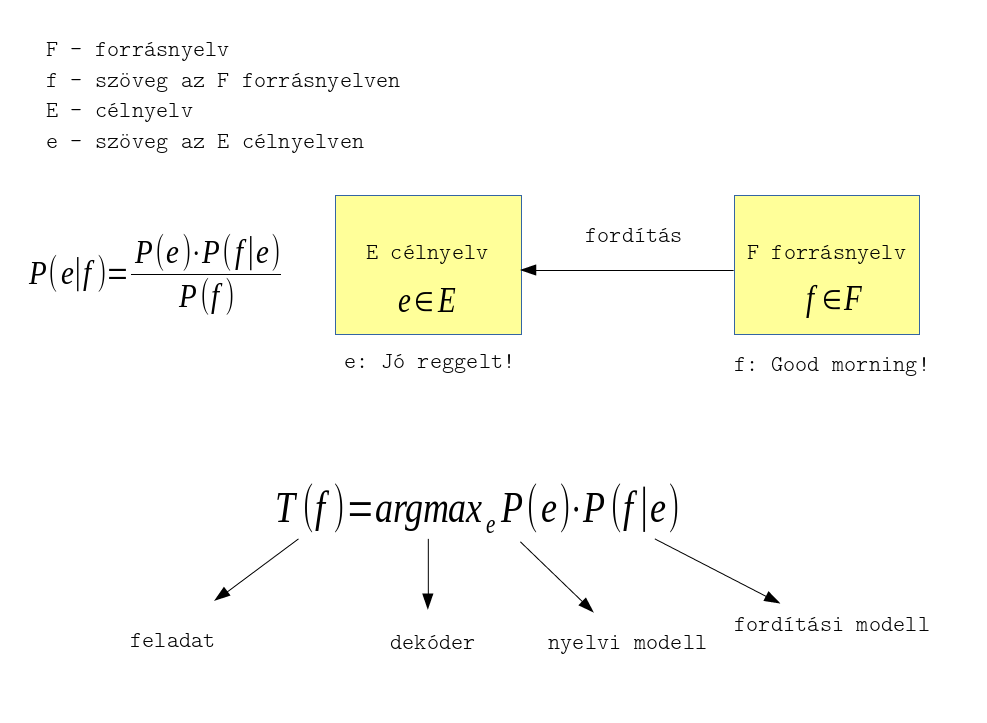
\includegraphics[width=1\linewidth]{images/smt}
  \end{figure}
\end{frame}

\begin{frame}{A statisztikus gépi fordítás alapjai}
  \begin{figure}[t]
  	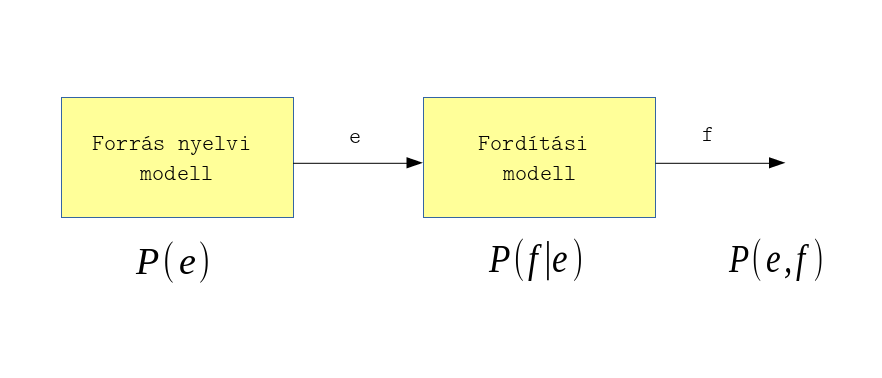
\includegraphics[width=1\linewidth]{images/smt2}
  \end{figure}
  
  \begin{itemize}
  	\item $P(e)$ nyelvi modell: n-gram modell
  	\item $P(f|e)$ fordítási modell: IBM modell
  	\item dekóder: StackDecoder
  \end{itemize}
\end{frame}

\begin{frame}{A nyelvi modell: bigrammok}
	\begin{itemize}
		\item Adva van egy angol szósorozat: $W = w_1,w_2,...,w_n$
		\item Lánc-szabály szerint: \begin{equation*}
		\begin{split}
		p(W) = p(w_1,w_2,...,w_n) = p(w_1) \cdot p(w_2|w_1) \cdot \\p(w_3|w_1, w_2) \cdot ... \cdot p(w_n|w_1,...,w_{n-1})
		\end{split}
		\end{equation*}
		\item \textbf{Markov-feltétel} bevezetése: a múlt legutolsó lépése számít
		\begin{equation*}
		\begin{split}
		p(w_1,w_2,...,w_n) = p(w_1) \cdot p(w_2|w_1) \cdot \\p(w_3|w_2) \cdot ... \cdot p(w_n|w_{n-1})
		\end{split}
		\end{equation*}
		\item ML-becslés: 
		\begin{equation*}
		p(w_2|w_1) = \frac{count(w_1,w_2)}{count(w_1)}
		\end{equation*}
	\end{itemize}
\end{frame}

\begin{frame}{IBM modell}

\end{frame}

\begin{frame}{StackDecoder}

\end{frame}